\PassOptionsToPackage{unicode=true}{hyperref} % options for packages loaded elsewhere
\PassOptionsToPackage{hyphens}{url}
\PassOptionsToPackage{dvipsnames,svgnames*,x11names*}{xcolor}
%
\documentclass[]{article}
\usepackage{lmodern}
\usepackage{amssymb,amsmath}
\usepackage{ifxetex,ifluatex}
\usepackage{fixltx2e} % provides \textsubscript
\ifnum 0\ifxetex 1\fi\ifluatex 1\fi=0 % if pdftex
  \usepackage[T1]{fontenc}
  \usepackage[utf8]{inputenc}
  \usepackage{textcomp} % provides euro and other symbols
\else % if luatex or xelatex
  \usepackage{unicode-math}
  \defaultfontfeatures{Ligatures=TeX,Scale=MatchLowercase}
\fi
% use upquote if available, for straight quotes in verbatim environments
\IfFileExists{upquote.sty}{\usepackage{upquote}}{}
% use microtype if available
\IfFileExists{microtype.sty}{%
\usepackage[]{microtype}
\UseMicrotypeSet[protrusion]{basicmath} % disable protrusion for tt fonts
}{}
\IfFileExists{parskip.sty}{%
\usepackage{parskip}
}{% else
\setlength{\parindent}{0pt}
\setlength{\parskip}{6pt plus 2pt minus 1pt}
}
\usepackage{xcolor}
\usepackage{hyperref}
\hypersetup{
            pdftitle={Taller datos FIFA 2019. Resuelto},
            colorlinks=true,
            linkcolor=red,
            filecolor=Maroon,
            citecolor=blue,
            urlcolor=blue,
            breaklinks=true}
\urlstyle{same}  % don't use monospace font for urls
\usepackage[margin=1in]{geometry}
\usepackage{color}
\usepackage{fancyvrb}
\newcommand{\VerbBar}{|}
\newcommand{\VERB}{\Verb[commandchars=\\\{\}]}
\DefineVerbatimEnvironment{Highlighting}{Verbatim}{commandchars=\\\{\}}
% Add ',fontsize=\small' for more characters per line
\usepackage{framed}
\definecolor{shadecolor}{RGB}{248,248,248}
\newenvironment{Shaded}{\begin{snugshade}}{\end{snugshade}}
\newcommand{\AlertTok}[1]{\textcolor[rgb]{0.94,0.16,0.16}{#1}}
\newcommand{\AnnotationTok}[1]{\textcolor[rgb]{0.56,0.35,0.01}{\textbf{\textit{#1}}}}
\newcommand{\AttributeTok}[1]{\textcolor[rgb]{0.77,0.63,0.00}{#1}}
\newcommand{\BaseNTok}[1]{\textcolor[rgb]{0.00,0.00,0.81}{#1}}
\newcommand{\BuiltInTok}[1]{#1}
\newcommand{\CharTok}[1]{\textcolor[rgb]{0.31,0.60,0.02}{#1}}
\newcommand{\CommentTok}[1]{\textcolor[rgb]{0.56,0.35,0.01}{\textit{#1}}}
\newcommand{\CommentVarTok}[1]{\textcolor[rgb]{0.56,0.35,0.01}{\textbf{\textit{#1}}}}
\newcommand{\ConstantTok}[1]{\textcolor[rgb]{0.00,0.00,0.00}{#1}}
\newcommand{\ControlFlowTok}[1]{\textcolor[rgb]{0.13,0.29,0.53}{\textbf{#1}}}
\newcommand{\DataTypeTok}[1]{\textcolor[rgb]{0.13,0.29,0.53}{#1}}
\newcommand{\DecValTok}[1]{\textcolor[rgb]{0.00,0.00,0.81}{#1}}
\newcommand{\DocumentationTok}[1]{\textcolor[rgb]{0.56,0.35,0.01}{\textbf{\textit{#1}}}}
\newcommand{\ErrorTok}[1]{\textcolor[rgb]{0.64,0.00,0.00}{\textbf{#1}}}
\newcommand{\ExtensionTok}[1]{#1}
\newcommand{\FloatTok}[1]{\textcolor[rgb]{0.00,0.00,0.81}{#1}}
\newcommand{\FunctionTok}[1]{\textcolor[rgb]{0.00,0.00,0.00}{#1}}
\newcommand{\ImportTok}[1]{#1}
\newcommand{\InformationTok}[1]{\textcolor[rgb]{0.56,0.35,0.01}{\textbf{\textit{#1}}}}
\newcommand{\KeywordTok}[1]{\textcolor[rgb]{0.13,0.29,0.53}{\textbf{#1}}}
\newcommand{\NormalTok}[1]{#1}
\newcommand{\OperatorTok}[1]{\textcolor[rgb]{0.81,0.36,0.00}{\textbf{#1}}}
\newcommand{\OtherTok}[1]{\textcolor[rgb]{0.56,0.35,0.01}{#1}}
\newcommand{\PreprocessorTok}[1]{\textcolor[rgb]{0.56,0.35,0.01}{\textit{#1}}}
\newcommand{\RegionMarkerTok}[1]{#1}
\newcommand{\SpecialCharTok}[1]{\textcolor[rgb]{0.00,0.00,0.00}{#1}}
\newcommand{\SpecialStringTok}[1]{\textcolor[rgb]{0.31,0.60,0.02}{#1}}
\newcommand{\StringTok}[1]{\textcolor[rgb]{0.31,0.60,0.02}{#1}}
\newcommand{\VariableTok}[1]{\textcolor[rgb]{0.00,0.00,0.00}{#1}}
\newcommand{\VerbatimStringTok}[1]{\textcolor[rgb]{0.31,0.60,0.02}{#1}}
\newcommand{\WarningTok}[1]{\textcolor[rgb]{0.56,0.35,0.01}{\textbf{\textit{#1}}}}
\usepackage{longtable,booktabs}
% Fix footnotes in tables (requires footnote package)
\IfFileExists{footnote.sty}{\usepackage{footnote}\makesavenoteenv{longtable}}{}
\usepackage{graphicx,grffile}
\makeatletter
\def\maxwidth{\ifdim\Gin@nat@width>\linewidth\linewidth\else\Gin@nat@width\fi}
\def\maxheight{\ifdim\Gin@nat@height>\textheight\textheight\else\Gin@nat@height\fi}
\makeatother
% Scale images if necessary, so that they will not overflow the page
% margins by default, and it is still possible to overwrite the defaults
% using explicit options in \includegraphics[width, height, ...]{}
\setkeys{Gin}{width=\maxwidth,height=\maxheight,keepaspectratio}
\setlength{\emergencystretch}{3em}  % prevent overfull lines
\providecommand{\tightlist}{%
  \setlength{\itemsep}{0pt}\setlength{\parskip}{0pt}}
\setcounter{secnumdepth}{5}
% Redefines (sub)paragraphs to behave more like sections
\ifx\paragraph\undefined\else
\let\oldparagraph\paragraph
\renewcommand{\paragraph}[1]{\oldparagraph{#1}\mbox{}}
\fi
\ifx\subparagraph\undefined\else
\let\oldsubparagraph\subparagraph
\renewcommand{\subparagraph}[1]{\oldsubparagraph{#1}\mbox{}}
\fi

% set default figure placement to htbp
\makeatletter
\def\fps@figure{htbp}
\makeatother

\renewcommand{\contentsname}{Contenidos}

\title{Taller datos FIFA 2019. Resuelto}
\author{}
\date{\vspace{-2.5em}25 marzo, 2022}

\begin{document}
\maketitle

{
\hypersetup{linkcolor=blue}
\setcounter{tocdepth}{2}
\tableofcontents
}
\hypertarget{taller-evaluable-datos-fifa-2020}{%
\section{Taller evaluable datos FIFA
2020}\label{taller-evaluable-datos-fifa-2020}}

Registraros en kaggle y bajaros el data set
\href{https://www.kaggle.com/stefanoleone992/fifa-20-complete-player-dataset}{FIFA
2020 Datos completos 2015 a 2020}. Guarda los datos en una carpeta
FIFA2020.

Las siguientes preguntas son relativas al data set
\texttt{players\_20.csv}.

Hay que contestar con código R explicar muy brevemente cada salida.
Subid a la activada el Rmd y el html.

Rellenad estos datos:

\textbf{PONED NOMBRE DEL GRUPO}

\begin{itemize}
\tightlist
\item
  Apellidos, Nombre Alumno
\end{itemize}

\hypertarget{pregunta-0}{%
\subsection{Pregunta 0}\label{pregunta-0}}

Explica el data set y de qué tipo son cada una de las variables y en qué
tipo de fichero están guardadas. Carga los datos en un data frame con
\texttt{read.csv} y explica las clases de cada columna de datos. Explica
el parámetro \texttt{encoding}. Es un data frame de 18278 observaciones
(filas) y 104 variables (columna).

Carga las variables de texto como factor \#\#\# Solución

\begin{Shaded}
\begin{Highlighting}[]
\NormalTok{datos =}\StringTok{ }\KeywordTok{read.csv}\NormalTok{(}\StringTok{"FIFA2020/players_20.csv"}\NormalTok{,}
  \DataTypeTok{encoding=}\StringTok{"UTF-8"}\NormalTok{,}\DataTypeTok{stringsAsFactors =} \OtherTok{TRUE}\NormalTok{)}\CommentTok{# cambia tu path}
\CommentTok{#str(datos)}
\CommentTok{#names(datos)}
\end{Highlighting}
\end{Shaded}

Las variables de la 1 (\texttt{sofifa\_id}) a la
31(\texttt{nation\_jersey\_number}) son variables de perfil del jugador:
su nombre, su equipo su sueldo su número de camiseta\ldots{} El resto de
variables de la 32 (\texttt{pace}) a la 104 (\texttt{rb}) son variables
numéricas enteras con valores de 0 a 100 que parametrizan cómo es el
jugador el el juego FIFA player 2020

\hypertarget{pregunta-1}{%
\subsection{Pregunta 1}\label{pregunta-1}}

¿Qué 6 clubs tienen a los 10 mejores jugadores según la variable
``shooting''?

\hypertarget{soluciuxf3n}{%
\subsubsection{Solución}\label{soluciuxf3n}}

La solución más adecuada es escoger los 10 mejores primeros jugadores
por la variable \texttt{shooting} los 6 primeros clubs. Pero como pueden
el Barça tiene dos juradores entre los 10 primeros hay que tomar los 6
mejores entre los clubs de los 10 mejores jugadores en \texttt{shooting}
sin repetir; eso lo conseguimos con la función \texttt{unique} o
simplemente construyendo la lista ala vista de los clubs de de los 10
mejores jugadores por \texttt{shooting} .

Se dará por correcta cualquier combinación de 6 clubs entre los clubs de
los 10 mejores jugadores por tiro a puerta \texttt{shooting}.

\begin{Shaded}
\begin{Highlighting}[]
\NormalTok{datos_o=datos[}\KeywordTok{order}\NormalTok{(datos}\OperatorTok{$}\NormalTok{shooting,}\DataTypeTok{decreasing=}\OtherTok{TRUE}\NormalTok{),]}
\NormalTok{datos_o}\OperatorTok{$}\NormalTok{shooting[}\DecValTok{1}\OperatorTok{:}\DecValTok{10}\NormalTok{]}
\end{Highlighting}
\end{Shaded}

\begin{verbatim}
##  [1] 93 92 91 90 89 89 88 88 87 87
\end{verbatim}

\begin{Shaded}
\begin{Highlighting}[]
\NormalTok{datos_o}\OperatorTok{$}\NormalTok{long_name[}\DecValTok{1}\OperatorTok{:}\DecValTok{10}\NormalTok{]}
\end{Highlighting}
\end{Shaded}

\begin{verbatim}
##  [1] Cristiano Ronaldo dos Santos Aveiro Lionel Andrés Messi Cuccittini     
##  [3] Harry Kane                          Sergio Leonel Agüero del Castillo  
##  [5] Luis Alberto Suárez Díaz            Fabio Quagliarella                 
##  [7] Marco Reus                          Zlatan Ibrahimović                 
##  [9] Robert Lewandowski                  Gareth Frank Bale                  
## 18218 Levels: A. Benjamin Chiamuloira Paes A. Pimenta Flora Pimenta ... 龙成
\end{verbatim}

\begin{Shaded}
\begin{Highlighting}[]
\NormalTok{datos_o}\OperatorTok{$}\NormalTok{club[}\DecValTok{1}\OperatorTok{:}\DecValTok{10}\NormalTok{]}
\end{Highlighting}
\end{Shaded}

\begin{verbatim}
##  [1] Juventus          FC Barcelona      Tottenham Hotspur Manchester City  
##  [5] FC Barcelona      Sampdoria         Borussia Dortmund LA Galaxy        
##  [9] FC Bayern München Real Madrid      
## 698 Levels:  SSV Jahn Regensburg 1. FC Heidenheim 1846 ... Zagłębie Lubin
\end{verbatim}

\begin{Shaded}
\begin{Highlighting}[]
\KeywordTok{unique}\NormalTok{(datos_o}\OperatorTok{$}\NormalTok{club)[}\DecValTok{1}\OperatorTok{:}\DecValTok{10}\NormalTok{]}
\end{Highlighting}
\end{Shaded}

\begin{verbatim}
##  [1] Juventus          FC Barcelona      Tottenham Hotspur Manchester City  
##  [5] Sampdoria         Borussia Dortmund LA Galaxy         FC Bayern München
##  [9] Real Madrid       Liverpool        
## 698 Levels:  SSV Jahn Regensburg 1. FC Heidenheim 1846 ... Zagłębie Lubin
\end{verbatim}

\begin{Shaded}
\begin{Highlighting}[]
\NormalTok{club6 =}\StringTok{ }\KeywordTok{unique}\NormalTok{(datos_o}\OperatorTok{$}\NormalTok{club)[}\DecValTok{1}\OperatorTok{:}\DecValTok{6}\NormalTok{]}\CommentTok{# así sacamos os 6 clubs o simplemente construyendo la lista}
\NormalTok{club6}
\end{Highlighting}
\end{Shaded}

\begin{verbatim}
## [1] Juventus          FC Barcelona      Tottenham Hotspur Manchester City  
## [5] Sampdoria         Borussia Dortmund
## 698 Levels:  SSV Jahn Regensburg 1. FC Heidenheim 1846 ... Zagłębie Lubin
\end{verbatim}

Notad que guardamos los nombres de los 6 clubs en la variable
\texttt{club6}.

\hypertarget{pregunta-2}{%
\subsection{Pregunta 2}\label{pregunta-2}}

Crea un data frame \texttt{fifa20\_best\_shooting} que contenga a TODOS
los jugadores de los clubs encontrados en el ejercicio anterior.

\hypertarget{soluciuxf3n-1}{%
\subsubsection{Solución}\label{soluciuxf3n-1}}

Construimos el data frame \texttt{fifa20\_best\_shooting} utilizando la
función \texttt{\%in\%} (estaba en el ejemplo de solución del profesor
del FIFA 2019). Se admite cualquier otra solución correcta.

\begin{Shaded}
\begin{Highlighting}[]
\NormalTok{fifa20_best_shooting=datos[datos}\OperatorTok{$}\NormalTok{club }\OperatorTok\StringTok{ }\NormalTok{club6,]}
\KeywordTok{unique}\NormalTok{(fifa20_best_shooting}\OperatorTok{$}\NormalTok{club)}
\end{Highlighting}
\end{Shaded}

\begin{verbatim}
## [1] FC Barcelona      Juventus          Manchester City   Tottenham Hotspur
## [5] Borussia Dortmund Sampdoria        
## 698 Levels:  SSV Jahn Regensburg 1. FC Heidenheim 1846 ... Zagłębie Lubin
\end{verbatim}

\hypertarget{pregunta-3}{%
\subsection{Pregunta 3}\label{pregunta-3}}

Calcular la media y la desviación típica del sueldo de cada equipo del
data frame \texttt{fifa20\_best\_shooting}.

\hypertarget{soluciuxf3n-2}{%
\subsubsection{Solución}\label{soluciuxf3n-2}}

Es una caso típico de uso de la función \texttt{aggregate} (es una
función clásica) está en el
\href{https://aprender-uib.github.io/AprendeR1/chap-df.html}{capítulo de
data frames de AprendeR1}.

\begin{Shaded}
\begin{Highlighting}[]
\KeywordTok{aggregate}\NormalTok{(wage_eur}\OperatorTok{~}\NormalTok{club, }\DataTypeTok{data=}\NormalTok{fifa20_best_shooting,}
          \DataTypeTok{FUN=}\ControlFlowTok{function}\NormalTok{(x)\{}\KeywordTok{c}\NormalTok{(}\DataTypeTok{media=}\KeywordTok{mean}\NormalTok{(x),}
                            \DataTypeTok{desv.tip=}\KeywordTok{sd}\NormalTok{(x),}
\NormalTok{                            mí}\DataTypeTok{nimo=}\KeywordTok{min}\NormalTok{(x),}
\NormalTok{                            má}\DataTypeTok{ximo=}\KeywordTok{max}\NormalTok{(x))\})}
\end{Highlighting}
\end{Shaded}

\begin{verbatim}
##                club wage_eur.media wage_eur.desv.tip wage_eur.mínimo
## 1 Borussia Dortmund       57806.45          43276.95         1000.00
## 2      FC Barcelona      150000.00         130914.81        12000.00
## 3          Juventus      113636.36          77462.42        17000.00
## 4   Manchester City      120727.27          99257.01         1000.00
## 5         Sampdoria       18781.25          11686.04         3000.00
## 6 Tottenham Hotspur       78878.79          60960.42         1000.00
##   wage_eur.máximo
## 1       170000.00
## 2       565000.00
## 3       405000.00
## 4       370000.00
## 5        46000.00
## 6       220000.00
\end{verbatim}

\hypertarget{pregunta-4}{%
\subsection{Pregunta 4}\label{pregunta-4}}

Discretiza la variable \texttt{age} de \texttt{fifa20\_best\_shooting}
en los 3 niveles siguientes: ``freshman'', ``junior'', ``senior'', según
los cortes por defecto. La variable resultante age\_Level tiene que ser
un factor ordenado en orden creciente de edad.

\hypertarget{soluciuxf3n-3}{%
\subsubsection{Solución}\label{soluciuxf3n-3}}

En el tema
\href{https://aprender-uib.github.io/AprendeR1/chap-hist.html}{Datos
cuantitativos agrupados de AprendeR1} se explica como agrupar variables
continuas por intervalos. En este caso nos piden la solución por defecto
de la función \texttt{cut}en 3 \texttt{breaks} y luego hay que
transformarla a un factor ordenado con los \texttt{levels} ``freshman'',
``junior'', ``senior''.

\begin{Shaded}
\begin{Highlighting}[]
\NormalTok{age3=}\KeywordTok{ordered}\NormalTok{(}\KeywordTok{cut}\NormalTok{(fifa20_best_shooting}\OperatorTok{$}\NormalTok{age,}\DataTypeTok{breaks=}\DecValTok{3}\NormalTok{))}\CommentTok{# corto en tres  partes}
\NormalTok{fifa20_best_shooting}\OperatorTok{$}\NormalTok{age[}\DecValTok{1}\OperatorTok{:}\DecValTok{10}\NormalTok{]}
\end{Highlighting}
\end{Shaded}

\begin{verbatim}
##  [1] 32 34 28 27 25 34 31 32 30 28
\end{verbatim}

\begin{Shaded}
\begin{Highlighting}[]
\NormalTok{age3[}\DecValTok{1}\OperatorTok{:}\DecValTok{10}\NormalTok{]}
\end{Highlighting}
\end{Shaded}

\begin{verbatim}
##  [1] (25,33] (33,41] (25,33] (25,33] (17,25] (33,41] (25,33] (25,33] (25,33]
## [10] (25,33]
## Levels: (17,25] < (25,33] < (33,41]
\end{verbatim}

\begin{Shaded}
\begin{Highlighting}[]
\KeywordTok{table}\NormalTok{(age3)}
\end{Highlighting}
\end{Shaded}

\begin{verbatim}
## age3
## (17,25] (25,33] (33,41] 
##     120      67       8
\end{verbatim}

\begin{Shaded}
\begin{Highlighting}[]
\KeywordTok{class}\NormalTok{(age3)}
\end{Highlighting}
\end{Shaded}

\begin{verbatim}
## [1] "ordered" "factor"
\end{verbatim}

\begin{Shaded}
\begin{Highlighting}[]
\KeywordTok{str}\NormalTok{(age3)}
\end{Highlighting}
\end{Shaded}

\begin{verbatim}
##  Ord.factor w/ 3 levels "(17,25]"<"(25,33]"<..: 2 3 2 2 1 3 2 2 2 2 ...
\end{verbatim}

\begin{Shaded}
\begin{Highlighting}[]
\KeywordTok{levels}\NormalTok{(age3)<-}\StringTok{ }\KeywordTok{c}\NormalTok{(}\StringTok{"freshman"}\NormalTok{, }\StringTok{"junior"}\NormalTok{, }\StringTok{"senior"}\NormalTok{)}
\KeywordTok{table}\NormalTok{(age3)}
\end{Highlighting}
\end{Shaded}

\begin{verbatim}
## age3
## freshman   junior   senior 
##      120       67        8
\end{verbatim}

\hypertarget{pregunta-5}{%
\subsection{Pregunta 5}\label{pregunta-5}}

¿Qué club tiene a más jugadores en el nivel ``senior'' calculado en el
ejercicio anterior?

\hypertarget{soluciuxf3n-4}{%
\subsubsection{Solución}\label{soluciuxf3n-4}}

\begin{Shaded}
\begin{Highlighting}[]
\KeywordTok{table}\NormalTok{(}\KeywordTok{droplevels}\NormalTok{(fifa20_best_shooting}\OperatorTok{$}\NormalTok{club),age3)}
\end{Highlighting}
\end{Shaded}

\begin{verbatim}
##                    age3
##                     freshman junior senior
##   Borussia Dortmund       20     10      1
##   FC Barcelona            21     12      0
##   Juventus                14     16      3
##   Manchester City         23      8      2
##   Sampdoria               22      8      2
##   Tottenham Hotspur       20     13      0
\end{verbatim}

Es el Juventus con 3 jugadores \texttt{senior}. Notad que utilizamos la
función \texttt{droplevels} para eliminar niveles de la variable club
que no aparecen en el data frame \texttt{fifa20\_best\_shooting}.

\hypertarget{pregunta-6}{%
\subsection{Pregunta 6}\label{pregunta-6}}

¿Cuántas nacionalidades hay entre todos los jugadores de
\texttt{fifa20\_best\_shooting}? ¿Qué club tiene mayor cantidad de
nacionalidades?

\hypertarget{soluciuxf3n-5}{%
\subsubsection{Solución}\label{soluciuxf3n-5}}

\begin{Shaded}
\begin{Highlighting}[]
\KeywordTok{length}\NormalTok{(}\KeywordTok{levels}\NormalTok{(fifa20_best_shooting}\OperatorTok{$}\NormalTok{nationality))}
\end{Highlighting}
\end{Shaded}

\begin{verbatim}
## [1] 162
\end{verbatim}

\begin{Shaded}
\begin{Highlighting}[]
\KeywordTok{length}\NormalTok{(}\KeywordTok{levels}\NormalTok{(fifa20_best_shooting}\OperatorTok{$}\NormalTok{nationality))}
\end{Highlighting}
\end{Shaded}

\begin{verbatim}
## [1] 162
\end{verbatim}

\begin{Shaded}
\begin{Highlighting}[]
\KeywordTok{length}\NormalTok{(}\KeywordTok{unique}\NormalTok{(}\KeywordTok{droplevels}\NormalTok{(fifa20_best_shooting}\OperatorTok{$}\NormalTok{nationality)))}
\end{Highlighting}
\end{Shaded}

\begin{verbatim}
## [1] 36
\end{verbatim}

Con esto sabemos que hay 36 nacionalidades distintas entre los 6 clubs.
Notemos que hemos combinado \texttt{droplevels}y \texttt{unique}para
obtener el resultado correcto.

Ahora contar las nacionalidades por club es un poco más delicado.
Podemos hacer la tabla de nacionalidades por club (como siempre con el
\texttt{droplevels})

\begin{Shaded}
\begin{Highlighting}[]
\NormalTok{knitr}\OperatorTok{::}\KeywordTok{kable}\NormalTok{(}
  \KeywordTok{t}\NormalTok{(}\KeywordTok{table}\NormalTok{(}\KeywordTok{droplevels}\NormalTok{(}
\NormalTok{    fifa20_best_shooting}\OperatorTok{$}\NormalTok{club),}
          \KeywordTok{droplevels}\NormalTok{(}
\NormalTok{            fifa20_best_shooting}\OperatorTok{$}\NormalTok{nationality)}
\NormalTok{    )}
\NormalTok{    ))}\CommentTok{# notad que transpongo la tabla }
\end{Highlighting}
\end{Shaded}

\begin{longtable}[]{@{}lrrrrrr@{}}
\toprule
\begin{minipage}[b]{0.16\columnwidth}\raggedright
\strut
\end{minipage} & \begin{minipage}[b]{0.14\columnwidth}\raggedleft
Borussia Dortmund\strut
\end{minipage} & \begin{minipage}[b]{0.10\columnwidth}\raggedleft
FC Barcelona\strut
\end{minipage} & \begin{minipage}[b]{0.07\columnwidth}\raggedleft
Juventus\strut
\end{minipage} & \begin{minipage}[b]{0.12\columnwidth}\raggedleft
Manchester City\strut
\end{minipage} & \begin{minipage}[b]{0.08\columnwidth}\raggedleft
Sampdoria\strut
\end{minipage} & \begin{minipage}[b]{0.14\columnwidth}\raggedleft
Tottenham Hotspur\strut
\end{minipage}\tabularnewline
\midrule
\endhead
\begin{minipage}[t]{0.16\columnwidth}\raggedright
Algeria\strut
\end{minipage} & \begin{minipage}[t]{0.14\columnwidth}\raggedleft
0\strut
\end{minipage} & \begin{minipage}[t]{0.10\columnwidth}\raggedleft
0\strut
\end{minipage} & \begin{minipage}[t]{0.07\columnwidth}\raggedleft
0\strut
\end{minipage} & \begin{minipage}[t]{0.12\columnwidth}\raggedleft
1\strut
\end{minipage} & \begin{minipage}[t]{0.08\columnwidth}\raggedleft
0\strut
\end{minipage} & \begin{minipage}[t]{0.14\columnwidth}\raggedleft
0\strut
\end{minipage}\tabularnewline
\begin{minipage}[t]{0.16\columnwidth}\raggedright
Argentina\strut
\end{minipage} & \begin{minipage}[t]{0.14\columnwidth}\raggedleft
1\strut
\end{minipage} & \begin{minipage}[t]{0.10\columnwidth}\raggedleft
1\strut
\end{minipage} & \begin{minipage}[t]{0.07\columnwidth}\raggedleft
2\strut
\end{minipage} & \begin{minipage}[t]{0.12\columnwidth}\raggedleft
3\strut
\end{minipage} & \begin{minipage}[t]{0.08\columnwidth}\raggedleft
1\strut
\end{minipage} & \begin{minipage}[t]{0.14\columnwidth}\raggedleft
4\strut
\end{minipage}\tabularnewline
\begin{minipage}[t]{0.16\columnwidth}\raggedright
Belgium\strut
\end{minipage} & \begin{minipage}[t]{0.14\columnwidth}\raggedleft
2\strut
\end{minipage} & \begin{minipage}[t]{0.10\columnwidth}\raggedleft
0\strut
\end{minipage} & \begin{minipage}[t]{0.07\columnwidth}\raggedleft
0\strut
\end{minipage} & \begin{minipage}[t]{0.12\columnwidth}\raggedleft
1\strut
\end{minipage} & \begin{minipage}[t]{0.08\columnwidth}\raggedleft
0\strut
\end{minipage} & \begin{minipage}[t]{0.14\columnwidth}\raggedleft
2\strut
\end{minipage}\tabularnewline
\begin{minipage}[t]{0.16\columnwidth}\raggedright
Bosnia Herzegovina\strut
\end{minipage} & \begin{minipage}[t]{0.14\columnwidth}\raggedleft
0\strut
\end{minipage} & \begin{minipage}[t]{0.10\columnwidth}\raggedleft
0\strut
\end{minipage} & \begin{minipage}[t]{0.07\columnwidth}\raggedleft
1\strut
\end{minipage} & \begin{minipage}[t]{0.12\columnwidth}\raggedleft
0\strut
\end{minipage} & \begin{minipage}[t]{0.08\columnwidth}\raggedleft
0\strut
\end{minipage} & \begin{minipage}[t]{0.14\columnwidth}\raggedleft
0\strut
\end{minipage}\tabularnewline
\begin{minipage}[t]{0.16\columnwidth}\raggedright
Brazil\strut
\end{minipage} & \begin{minipage}[t]{0.14\columnwidth}\raggedleft
0\strut
\end{minipage} & \begin{minipage}[t]{0.10\columnwidth}\raggedleft
3\strut
\end{minipage} & \begin{minipage}[t]{0.07\columnwidth}\raggedleft
4\strut
\end{minipage} & \begin{minipage}[t]{0.12\columnwidth}\raggedleft
3\strut
\end{minipage} & \begin{minipage}[t]{0.08\columnwidth}\raggedleft
0\strut
\end{minipage} & \begin{minipage}[t]{0.14\columnwidth}\raggedleft
1\strut
\end{minipage}\tabularnewline
\begin{minipage}[t]{0.16\columnwidth}\raggedright
Chile\strut
\end{minipage} & \begin{minipage}[t]{0.14\columnwidth}\raggedleft
0\strut
\end{minipage} & \begin{minipage}[t]{0.10\columnwidth}\raggedleft
1\strut
\end{minipage} & \begin{minipage}[t]{0.07\columnwidth}\raggedleft
0\strut
\end{minipage} & \begin{minipage}[t]{0.12\columnwidth}\raggedleft
1\strut
\end{minipage} & \begin{minipage}[t]{0.08\columnwidth}\raggedleft
0\strut
\end{minipage} & \begin{minipage}[t]{0.14\columnwidth}\raggedleft
0\strut
\end{minipage}\tabularnewline
\begin{minipage}[t]{0.16\columnwidth}\raggedright
Colombia\strut
\end{minipage} & \begin{minipage}[t]{0.14\columnwidth}\raggedleft
0\strut
\end{minipage} & \begin{minipage}[t]{0.10\columnwidth}\raggedleft
0\strut
\end{minipage} & \begin{minipage}[t]{0.07\columnwidth}\raggedleft
1\strut
\end{minipage} & \begin{minipage}[t]{0.12\columnwidth}\raggedleft
0\strut
\end{minipage} & \begin{minipage}[t]{0.08\columnwidth}\raggedleft
1\strut
\end{minipage} & \begin{minipage}[t]{0.14\columnwidth}\raggedleft
1\strut
\end{minipage}\tabularnewline
\begin{minipage}[t]{0.16\columnwidth}\raggedright
Croatia\strut
\end{minipage} & \begin{minipage}[t]{0.14\columnwidth}\raggedleft
0\strut
\end{minipage} & \begin{minipage}[t]{0.10\columnwidth}\raggedleft
1\strut
\end{minipage} & \begin{minipage}[t]{0.07\columnwidth}\raggedleft
2\strut
\end{minipage} & \begin{minipage}[t]{0.12\columnwidth}\raggedleft
0\strut
\end{minipage} & \begin{minipage}[t]{0.08\columnwidth}\raggedleft
0\strut
\end{minipage} & \begin{minipage}[t]{0.14\columnwidth}\raggedleft
0\strut
\end{minipage}\tabularnewline
\begin{minipage}[t]{0.16\columnwidth}\raggedright
Cyprus\strut
\end{minipage} & \begin{minipage}[t]{0.14\columnwidth}\raggedleft
0\strut
\end{minipage} & \begin{minipage}[t]{0.10\columnwidth}\raggedleft
0\strut
\end{minipage} & \begin{minipage}[t]{0.07\columnwidth}\raggedleft
0\strut
\end{minipage} & \begin{minipage}[t]{0.12\columnwidth}\raggedleft
0\strut
\end{minipage} & \begin{minipage}[t]{0.08\columnwidth}\raggedleft
0\strut
\end{minipage} & \begin{minipage}[t]{0.14\columnwidth}\raggedleft
2\strut
\end{minipage}\tabularnewline
\begin{minipage}[t]{0.16\columnwidth}\raggedright
Czech Republic\strut
\end{minipage} & \begin{minipage}[t]{0.14\columnwidth}\raggedleft
0\strut
\end{minipage} & \begin{minipage}[t]{0.10\columnwidth}\raggedleft
0\strut
\end{minipage} & \begin{minipage}[t]{0.07\columnwidth}\raggedleft
0\strut
\end{minipage} & \begin{minipage}[t]{0.12\columnwidth}\raggedleft
0\strut
\end{minipage} & \begin{minipage}[t]{0.08\columnwidth}\raggedleft
1\strut
\end{minipage} & \begin{minipage}[t]{0.14\columnwidth}\raggedleft
0\strut
\end{minipage}\tabularnewline
\begin{minipage}[t]{0.16\columnwidth}\raggedright
Denmark\strut
\end{minipage} & \begin{minipage}[t]{0.14\columnwidth}\raggedleft
2\strut
\end{minipage} & \begin{minipage}[t]{0.10\columnwidth}\raggedleft
0\strut
\end{minipage} & \begin{minipage}[t]{0.07\columnwidth}\raggedleft
0\strut
\end{minipage} & \begin{minipage}[t]{0.12\columnwidth}\raggedleft
0\strut
\end{minipage} & \begin{minipage}[t]{0.08\columnwidth}\raggedleft
0\strut
\end{minipage} & \begin{minipage}[t]{0.14\columnwidth}\raggedleft
1\strut
\end{minipage}\tabularnewline
\begin{minipage}[t]{0.16\columnwidth}\raggedright
England\strut
\end{minipage} & \begin{minipage}[t]{0.14\columnwidth}\raggedleft
1\strut
\end{minipage} & \begin{minipage}[t]{0.10\columnwidth}\raggedleft
0\strut
\end{minipage} & \begin{minipage}[t]{0.07\columnwidth}\raggedleft
0\strut
\end{minipage} & \begin{minipage}[t]{0.12\columnwidth}\raggedleft
8\strut
\end{minipage} & \begin{minipage}[t]{0.08\columnwidth}\raggedleft
1\strut
\end{minipage} & \begin{minipage}[t]{0.14\columnwidth}\raggedleft
13\strut
\end{minipage}\tabularnewline
\begin{minipage}[t]{0.16\columnwidth}\raggedright
France\strut
\end{minipage} & \begin{minipage}[t]{0.14\columnwidth}\raggedleft
2\strut
\end{minipage} & \begin{minipage}[t]{0.10\columnwidth}\raggedleft
5\strut
\end{minipage} & \begin{minipage}[t]{0.07\columnwidth}\raggedleft
3\strut
\end{minipage} & \begin{minipage}[t]{0.12\columnwidth}\raggedleft
3\strut
\end{minipage} & \begin{minipage}[t]{0.08\columnwidth}\raggedleft
2\strut
\end{minipage} & \begin{minipage}[t]{0.14\columnwidth}\raggedleft
4\strut
\end{minipage}\tabularnewline
\begin{minipage}[t]{0.16\columnwidth}\raggedright
Gambia\strut
\end{minipage} & \begin{minipage}[t]{0.14\columnwidth}\raggedleft
0\strut
\end{minipage} & \begin{minipage}[t]{0.10\columnwidth}\raggedleft
0\strut
\end{minipage} & \begin{minipage}[t]{0.07\columnwidth}\raggedleft
0\strut
\end{minipage} & \begin{minipage}[t]{0.12\columnwidth}\raggedleft
0\strut
\end{minipage} & \begin{minipage}[t]{0.08\columnwidth}\raggedleft
1\strut
\end{minipage} & \begin{minipage}[t]{0.14\columnwidth}\raggedleft
0\strut
\end{minipage}\tabularnewline
\begin{minipage}[t]{0.16\columnwidth}\raggedright
Germany\strut
\end{minipage} & \begin{minipage}[t]{0.14\columnwidth}\raggedleft
15\strut
\end{minipage} & \begin{minipage}[t]{0.10\columnwidth}\raggedleft
1\strut
\end{minipage} & \begin{minipage}[t]{0.07\columnwidth}\raggedleft
2\strut
\end{minipage} & \begin{minipage}[t]{0.12\columnwidth}\raggedleft
2\strut
\end{minipage} & \begin{minipage}[t]{0.08\columnwidth}\raggedleft
1\strut
\end{minipage} & \begin{minipage}[t]{0.14\columnwidth}\raggedleft
0\strut
\end{minipage}\tabularnewline
\begin{minipage}[t]{0.16\columnwidth}\raggedright
Italy\strut
\end{minipage} & \begin{minipage}[t]{0.14\columnwidth}\raggedleft
0\strut
\end{minipage} & \begin{minipage}[t]{0.10\columnwidth}\raggedleft
0\strut
\end{minipage} & \begin{minipage}[t]{0.07\columnwidth}\raggedleft
12\strut
\end{minipage} & \begin{minipage}[t]{0.12\columnwidth}\raggedleft
0\strut
\end{minipage} & \begin{minipage}[t]{0.08\columnwidth}\raggedleft
17\strut
\end{minipage} & \begin{minipage}[t]{0.14\columnwidth}\raggedleft
0\strut
\end{minipage}\tabularnewline
\begin{minipage}[t]{0.16\columnwidth}\raggedright
Ivory Coast\strut
\end{minipage} & \begin{minipage}[t]{0.14\columnwidth}\raggedleft
0\strut
\end{minipage} & \begin{minipage}[t]{0.10\columnwidth}\raggedleft
0\strut
\end{minipage} & \begin{minipage}[t]{0.07\columnwidth}\raggedleft
0\strut
\end{minipage} & \begin{minipage}[t]{0.12\columnwidth}\raggedleft
0\strut
\end{minipage} & \begin{minipage}[t]{0.08\columnwidth}\raggedleft
0\strut
\end{minipage} & \begin{minipage}[t]{0.14\columnwidth}\raggedleft
1\strut
\end{minipage}\tabularnewline
\begin{minipage}[t]{0.16\columnwidth}\raggedright
Japan\strut
\end{minipage} & \begin{minipage}[t]{0.14\columnwidth}\raggedleft
0\strut
\end{minipage} & \begin{minipage}[t]{0.10\columnwidth}\raggedleft
1\strut
\end{minipage} & \begin{minipage}[t]{0.07\columnwidth}\raggedleft
0\strut
\end{minipage} & \begin{minipage}[t]{0.12\columnwidth}\raggedleft
0\strut
\end{minipage} & \begin{minipage}[t]{0.08\columnwidth}\raggedleft
0\strut
\end{minipage} & \begin{minipage}[t]{0.14\columnwidth}\raggedleft
0\strut
\end{minipage}\tabularnewline
\begin{minipage}[t]{0.16\columnwidth}\raggedright
Kenya\strut
\end{minipage} & \begin{minipage}[t]{0.14\columnwidth}\raggedleft
0\strut
\end{minipage} & \begin{minipage}[t]{0.10\columnwidth}\raggedleft
0\strut
\end{minipage} & \begin{minipage}[t]{0.07\columnwidth}\raggedleft
0\strut
\end{minipage} & \begin{minipage}[t]{0.12\columnwidth}\raggedleft
0\strut
\end{minipage} & \begin{minipage}[t]{0.08\columnwidth}\raggedleft
0\strut
\end{minipage} & \begin{minipage}[t]{0.14\columnwidth}\raggedleft
1\strut
\end{minipage}\tabularnewline
\begin{minipage}[t]{0.16\columnwidth}\raggedright
Korea Republic\strut
\end{minipage} & \begin{minipage}[t]{0.14\columnwidth}\raggedleft
0\strut
\end{minipage} & \begin{minipage}[t]{0.10\columnwidth}\raggedleft
0\strut
\end{minipage} & \begin{minipage}[t]{0.07\columnwidth}\raggedleft
0\strut
\end{minipage} & \begin{minipage}[t]{0.12\columnwidth}\raggedleft
0\strut
\end{minipage} & \begin{minipage}[t]{0.08\columnwidth}\raggedleft
0\strut
\end{minipage} & \begin{minipage}[t]{0.14\columnwidth}\raggedleft
1\strut
\end{minipage}\tabularnewline
\begin{minipage}[t]{0.16\columnwidth}\raggedright
Montenegro\strut
\end{minipage} & \begin{minipage}[t]{0.14\columnwidth}\raggedleft
0\strut
\end{minipage} & \begin{minipage}[t]{0.10\columnwidth}\raggedleft
0\strut
\end{minipage} & \begin{minipage}[t]{0.07\columnwidth}\raggedleft
0\strut
\end{minipage} & \begin{minipage}[t]{0.12\columnwidth}\raggedleft
0\strut
\end{minipage} & \begin{minipage}[t]{0.08\columnwidth}\raggedleft
1\strut
\end{minipage} & \begin{minipage}[t]{0.14\columnwidth}\raggedleft
0\strut
\end{minipage}\tabularnewline
\begin{minipage}[t]{0.16\columnwidth}\raggedright
Morocco\strut
\end{minipage} & \begin{minipage}[t]{0.14\columnwidth}\raggedleft
1\strut
\end{minipage} & \begin{minipage}[t]{0.10\columnwidth}\raggedleft
0\strut
\end{minipage} & \begin{minipage}[t]{0.07\columnwidth}\raggedleft
0\strut
\end{minipage} & \begin{minipage}[t]{0.12\columnwidth}\raggedleft
0\strut
\end{minipage} & \begin{minipage}[t]{0.08\columnwidth}\raggedleft
0\strut
\end{minipage} & \begin{minipage}[t]{0.14\columnwidth}\raggedleft
0\strut
\end{minipage}\tabularnewline
\begin{minipage}[t]{0.16\columnwidth}\raggedright
Netherlands\strut
\end{minipage} & \begin{minipage}[t]{0.14\columnwidth}\raggedleft
0\strut
\end{minipage} & \begin{minipage}[t]{0.10\columnwidth}\raggedleft
2\strut
\end{minipage} & \begin{minipage}[t]{0.07\columnwidth}\raggedleft
1\strut
\end{minipage} & \begin{minipage}[t]{0.12\columnwidth}\raggedleft
0\strut
\end{minipage} & \begin{minipage}[t]{0.08\columnwidth}\raggedleft
0\strut
\end{minipage} & \begin{minipage}[t]{0.14\columnwidth}\raggedleft
0\strut
\end{minipage}\tabularnewline
\begin{minipage}[t]{0.16\columnwidth}\raggedright
Norway\strut
\end{minipage} & \begin{minipage}[t]{0.14\columnwidth}\raggedleft
0\strut
\end{minipage} & \begin{minipage}[t]{0.10\columnwidth}\raggedleft
0\strut
\end{minipage} & \begin{minipage}[t]{0.07\columnwidth}\raggedleft
0\strut
\end{minipage} & \begin{minipage}[t]{0.12\columnwidth}\raggedleft
0\strut
\end{minipage} & \begin{minipage}[t]{0.08\columnwidth}\raggedleft
1\strut
\end{minipage} & \begin{minipage}[t]{0.14\columnwidth}\raggedleft
0\strut
\end{minipage}\tabularnewline
\begin{minipage}[t]{0.16\columnwidth}\raggedright
Paraguay\strut
\end{minipage} & \begin{minipage}[t]{0.14\columnwidth}\raggedleft
0\strut
\end{minipage} & \begin{minipage}[t]{0.10\columnwidth}\raggedleft
0\strut
\end{minipage} & \begin{minipage}[t]{0.07\columnwidth}\raggedleft
0\strut
\end{minipage} & \begin{minipage}[t]{0.12\columnwidth}\raggedleft
0\strut
\end{minipage} & \begin{minipage}[t]{0.08\columnwidth}\raggedleft
1\strut
\end{minipage} & \begin{minipage}[t]{0.14\columnwidth}\raggedleft
0\strut
\end{minipage}\tabularnewline
\begin{minipage}[t]{0.16\columnwidth}\raggedright
Poland\strut
\end{minipage} & \begin{minipage}[t]{0.14\columnwidth}\raggedleft
1\strut
\end{minipage} & \begin{minipage}[t]{0.10\columnwidth}\raggedleft
0\strut
\end{minipage} & \begin{minipage}[t]{0.07\columnwidth}\raggedleft
1\strut
\end{minipage} & \begin{minipage}[t]{0.12\columnwidth}\raggedleft
0\strut
\end{minipage} & \begin{minipage}[t]{0.08\columnwidth}\raggedleft
2\strut
\end{minipage} & \begin{minipage}[t]{0.14\columnwidth}\raggedleft
0\strut
\end{minipage}\tabularnewline
\begin{minipage}[t]{0.16\columnwidth}\raggedright
Portugal\strut
\end{minipage} & \begin{minipage}[t]{0.14\columnwidth}\raggedleft
1\strut
\end{minipage} & \begin{minipage}[t]{0.10\columnwidth}\raggedleft
1\strut
\end{minipage} & \begin{minipage}[t]{0.07\columnwidth}\raggedleft
1\strut
\end{minipage} & \begin{minipage}[t]{0.12\columnwidth}\raggedleft
2\strut
\end{minipage} & \begin{minipage}[t]{0.08\columnwidth}\raggedleft
0\strut
\end{minipage} & \begin{minipage}[t]{0.14\columnwidth}\raggedleft
0\strut
\end{minipage}\tabularnewline
\begin{minipage}[t]{0.16\columnwidth}\raggedright
Republic of Ireland\strut
\end{minipage} & \begin{minipage}[t]{0.14\columnwidth}\raggedleft
0\strut
\end{minipage} & \begin{minipage}[t]{0.10\columnwidth}\raggedleft
0\strut
\end{minipage} & \begin{minipage}[t]{0.07\columnwidth}\raggedleft
0\strut
\end{minipage} & \begin{minipage}[t]{0.12\columnwidth}\raggedleft
2\strut
\end{minipage} & \begin{minipage}[t]{0.08\columnwidth}\raggedleft
0\strut
\end{minipage} & \begin{minipage}[t]{0.14\columnwidth}\raggedleft
1\strut
\end{minipage}\tabularnewline
\begin{minipage}[t]{0.16\columnwidth}\raggedright
Senegal\strut
\end{minipage} & \begin{minipage}[t]{0.14\columnwidth}\raggedleft
0\strut
\end{minipage} & \begin{minipage}[t]{0.10\columnwidth}\raggedleft
1\strut
\end{minipage} & \begin{minipage}[t]{0.07\columnwidth}\raggedleft
0\strut
\end{minipage} & \begin{minipage}[t]{0.12\columnwidth}\raggedleft
0\strut
\end{minipage} & \begin{minipage}[t]{0.08\columnwidth}\raggedleft
0\strut
\end{minipage} & \begin{minipage}[t]{0.14\columnwidth}\raggedleft
0\strut
\end{minipage}\tabularnewline
\begin{minipage}[t]{0.16\columnwidth}\raggedright
Spain\strut
\end{minipage} & \begin{minipage}[t]{0.14\columnwidth}\raggedleft
2\strut
\end{minipage} & \begin{minipage}[t]{0.10\columnwidth}\raggedleft
15\strut
\end{minipage} & \begin{minipage}[t]{0.07\columnwidth}\raggedleft
0\strut
\end{minipage} & \begin{minipage}[t]{0.12\columnwidth}\raggedleft
5\strut
\end{minipage} & \begin{minipage}[t]{0.08\columnwidth}\raggedleft
0\strut
\end{minipage} & \begin{minipage}[t]{0.14\columnwidth}\raggedleft
0\strut
\end{minipage}\tabularnewline
\begin{minipage}[t]{0.16\columnwidth}\raggedright
Sweden\strut
\end{minipage} & \begin{minipage}[t]{0.14\columnwidth}\raggedleft
0\strut
\end{minipage} & \begin{minipage}[t]{0.10\columnwidth}\raggedleft
0\strut
\end{minipage} & \begin{minipage}[t]{0.07\columnwidth}\raggedleft
0\strut
\end{minipage} & \begin{minipage}[t]{0.12\columnwidth}\raggedleft
0\strut
\end{minipage} & \begin{minipage}[t]{0.08\columnwidth}\raggedleft
1\strut
\end{minipage} & \begin{minipage}[t]{0.14\columnwidth}\raggedleft
0\strut
\end{minipage}\tabularnewline
\begin{minipage}[t]{0.16\columnwidth}\raggedright
Switzerland\strut
\end{minipage} & \begin{minipage}[t]{0.14\columnwidth}\raggedleft
3\strut
\end{minipage} & \begin{minipage}[t]{0.10\columnwidth}\raggedleft
0\strut
\end{minipage} & \begin{minipage}[t]{0.07\columnwidth}\raggedleft
0\strut
\end{minipage} & \begin{minipage}[t]{0.12\columnwidth}\raggedleft
1\strut
\end{minipage} & \begin{minipage}[t]{0.08\columnwidth}\raggedleft
0\strut
\end{minipage} & \begin{minipage}[t]{0.14\columnwidth}\raggedleft
0\strut
\end{minipage}\tabularnewline
\begin{minipage}[t]{0.16\columnwidth}\raggedright
Turkey\strut
\end{minipage} & \begin{minipage}[t]{0.14\columnwidth}\raggedleft
0\strut
\end{minipage} & \begin{minipage}[t]{0.10\columnwidth}\raggedleft
0\strut
\end{minipage} & \begin{minipage}[t]{0.07\columnwidth}\raggedleft
1\strut
\end{minipage} & \begin{minipage}[t]{0.12\columnwidth}\raggedleft
0\strut
\end{minipage} & \begin{minipage}[t]{0.08\columnwidth}\raggedleft
0\strut
\end{minipage} & \begin{minipage}[t]{0.14\columnwidth}\raggedleft
0\strut
\end{minipage}\tabularnewline
\begin{minipage}[t]{0.16\columnwidth}\raggedright
Ukraine\strut
\end{minipage} & \begin{minipage}[t]{0.14\columnwidth}\raggedleft
0\strut
\end{minipage} & \begin{minipage}[t]{0.10\columnwidth}\raggedleft
0\strut
\end{minipage} & \begin{minipage}[t]{0.07\columnwidth}\raggedleft
0\strut
\end{minipage} & \begin{minipage}[t]{0.12\columnwidth}\raggedleft
1\strut
\end{minipage} & \begin{minipage}[t]{0.08\columnwidth}\raggedleft
0\strut
\end{minipage} & \begin{minipage}[t]{0.14\columnwidth}\raggedleft
0\strut
\end{minipage}\tabularnewline
\begin{minipage}[t]{0.16\columnwidth}\raggedright
Uruguay\strut
\end{minipage} & \begin{minipage}[t]{0.14\columnwidth}\raggedleft
0\strut
\end{minipage} & \begin{minipage}[t]{0.10\columnwidth}\raggedleft
1\strut
\end{minipage} & \begin{minipage}[t]{0.07\columnwidth}\raggedleft
1\strut
\end{minipage} & \begin{minipage}[t]{0.12\columnwidth}\raggedleft
0\strut
\end{minipage} & \begin{minipage}[t]{0.08\columnwidth}\raggedleft
1\strut
\end{minipage} & \begin{minipage}[t]{0.14\columnwidth}\raggedleft
0\strut
\end{minipage}\tabularnewline
\begin{minipage}[t]{0.16\columnwidth}\raggedright
Wales\strut
\end{minipage} & \begin{minipage}[t]{0.14\columnwidth}\raggedleft
0\strut
\end{minipage} & \begin{minipage}[t]{0.10\columnwidth}\raggedleft
0\strut
\end{minipage} & \begin{minipage}[t]{0.07\columnwidth}\raggedleft
1\strut
\end{minipage} & \begin{minipage}[t]{0.12\columnwidth}\raggedleft
0\strut
\end{minipage} & \begin{minipage}[t]{0.08\columnwidth}\raggedleft
0\strut
\end{minipage} & \begin{minipage}[t]{0.14\columnwidth}\raggedleft
1\strut
\end{minipage}\tabularnewline
\bottomrule
\end{longtable}

\begin{Shaded}
\begin{Highlighting}[]
\CommentTok{# como si fuera una matriz con la función t.}
\end{Highlighting}
\end{Shaded}

y luego marcar las nacionalidades \(>0\) con una variable lógica y
acumular la tabla por filas con \texttt{rowSums}.

\begin{Shaded}
\begin{Highlighting}[]
\NormalTok{nac_por_club=}\KeywordTok{table}\NormalTok{(}\KeywordTok{droplevels}\NormalTok{(fifa20_best_shooting}\OperatorTok{$}\NormalTok{club),}\KeywordTok{droplevels}\NormalTok{(fifa20_best_shooting}\OperatorTok{$}\NormalTok{nationality))}
\NormalTok{aux=nac_por_club}\OperatorTok{>}\DecValTok{0}
\KeywordTok{rowSums}\NormalTok{(aux)}
\end{Highlighting}
\end{Shaded}

\begin{verbatim}
## Borussia Dortmund      FC Barcelona          Juventus   Manchester City 
##                11                12                14                13 
##         Sampdoria Tottenham Hotspur 
##                14                13
\end{verbatim}

Así obtenemos el número de nacionalidades por club.

\hypertarget{pregunta-7}{%
\subsection{Pregunta 7}\label{pregunta-7}}

Calcula mediante un diagrama de barras ordenado de mayor a menor la
proporción de jugadores de cada nacionalidad en cada club

\hypertarget{soluciuxf3n-6}{%
\subsubsection{Solución}\label{soluciuxf3n-6}}

He viso innumerables soluciones. Si habéis conseguido las gráficas
correctas y pues to el título las puntuaremos como correctas.

Yo doy esta solución (he utilizado un \texttt{for} que es del tema
\href{https://aprender-uib.github.io/AprendeR1/chap-for.html}{Estructuta
de control básicas de AprendeR1})

Construyo una función que me da la nacionalidad por club y dibujo los
\texttt{barplot} con el título y nombres adecuados.

\begin{Shaded}
\begin{Highlighting}[]
\NormalTok{porcen_nac_por_club=}\DecValTok{100}\OperatorTok{*}\KeywordTok{prop.table}\NormalTok{(nac_por_club,}\DataTypeTok{margin=}\DecValTok{1}\NormalTok{)}
\NormalTok{nombre_club=}\KeywordTok{as.character}\NormalTok{(club6)}
\NormalTok{nombre_club}
\end{Highlighting}
\end{Shaded}

\begin{verbatim}
## [1] "Juventus"          "FC Barcelona"      "Tottenham Hotspur"
## [4] "Manchester City"   "Sampdoria"         "Borussia Dortmund"
\end{verbatim}

\begin{Shaded}
\begin{Highlighting}[]
\ControlFlowTok{for}\NormalTok{(i }\ControlFlowTok{in} \DecValTok{1}\OperatorTok{:}\DecValTok{6}\NormalTok{)\{}
\NormalTok{  alturas=}\KeywordTok{sort}\NormalTok{(porcen_nac_por_club[i,],}\DataTypeTok{decreasing=}\OtherTok{TRUE}\NormalTok{)}
\KeywordTok{barplot}\NormalTok{(alturas,}
        \DataTypeTok{ylim=}\KeywordTok{c}\NormalTok{(}\DecValTok{0}\NormalTok{,}\KeywordTok{max}\NormalTok{(alturas)}\OperatorTok{+}\DecValTok{10}\NormalTok{),}
               \DataTypeTok{las=}\DecValTok{2}\NormalTok{,}\DataTypeTok{cex.names=}\FloatTok{0.8}\NormalTok{,}\DataTypeTok{ylab=}\StringTok{"Porcentaje %"}\NormalTok{,}
        \DataTypeTok{main=}\KeywordTok{paste0}\NormalTok{(}\KeywordTok{c}\NormalTok{(}\StringTok{"Porcentaje nacionalidades}\CharTok{\textbackslash{}n}\StringTok{"}\NormalTok{,nombre_club[i])),}\DataTypeTok{col=}\StringTok{"blue"}\NormalTok{)}
\NormalTok{\}}
\end{Highlighting}
\end{Shaded}

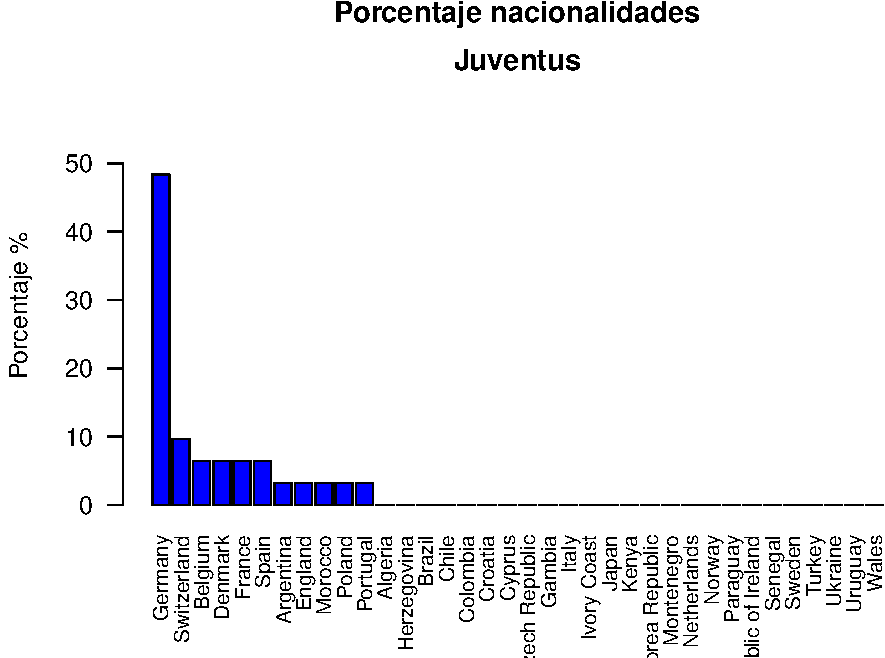
\includegraphics{taller_FIFA_SOLUCION_files/figure-latex/unnamed-chunk-9-1.pdf}
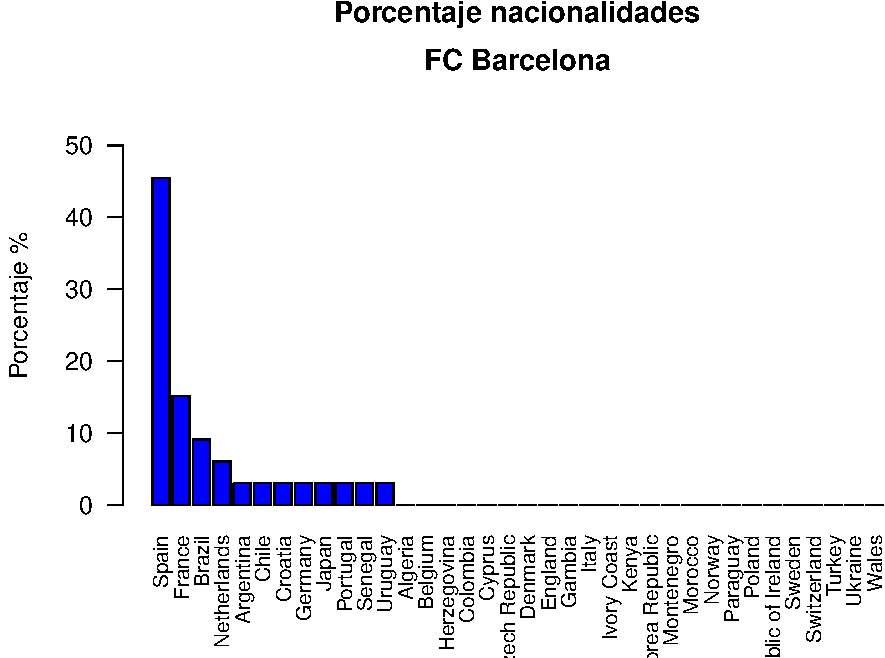
\includegraphics{taller_FIFA_SOLUCION_files/figure-latex/unnamed-chunk-9-2.pdf}
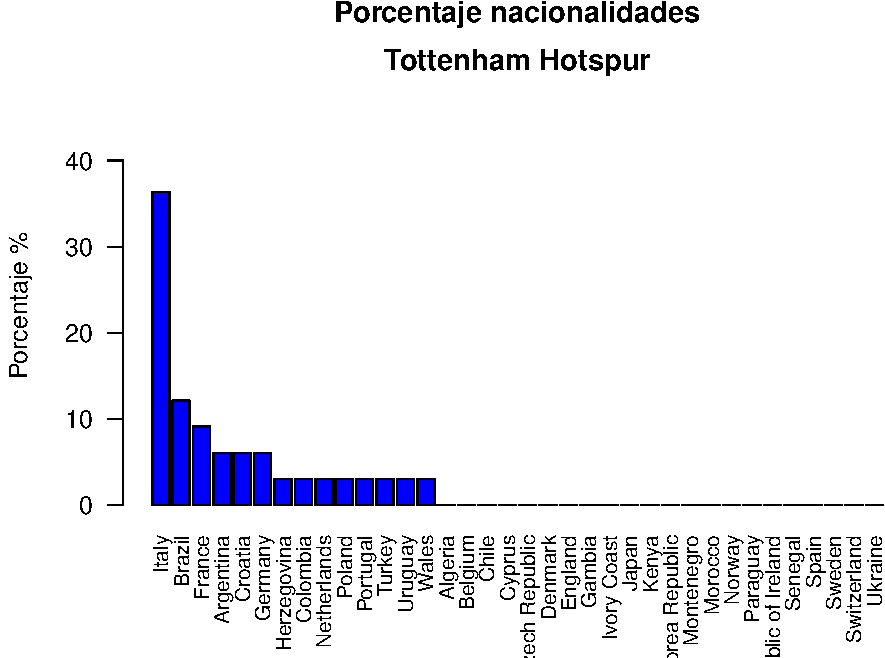
\includegraphics{taller_FIFA_SOLUCION_files/figure-latex/unnamed-chunk-9-3.pdf}
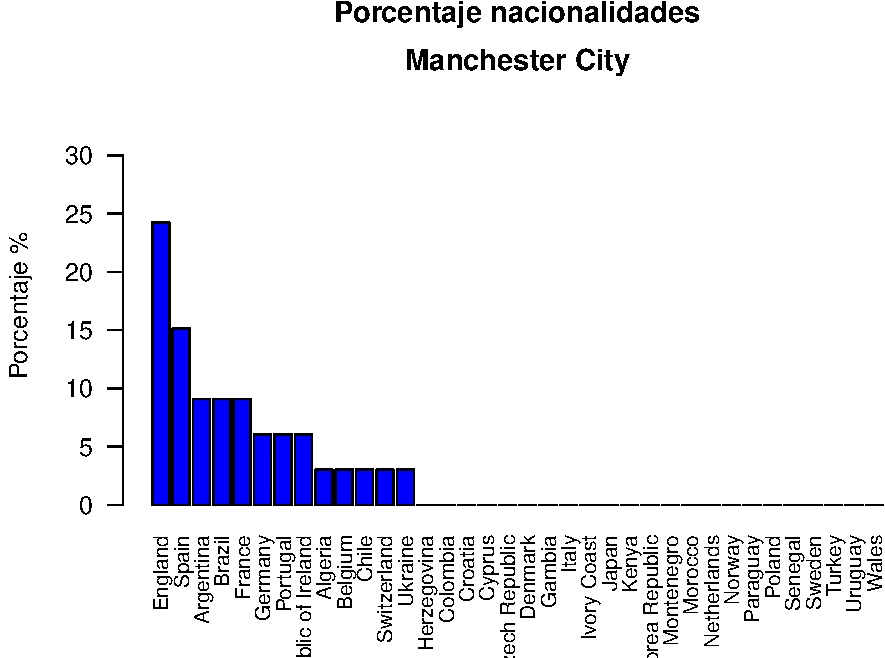
\includegraphics{taller_FIFA_SOLUCION_files/figure-latex/unnamed-chunk-9-4.pdf}
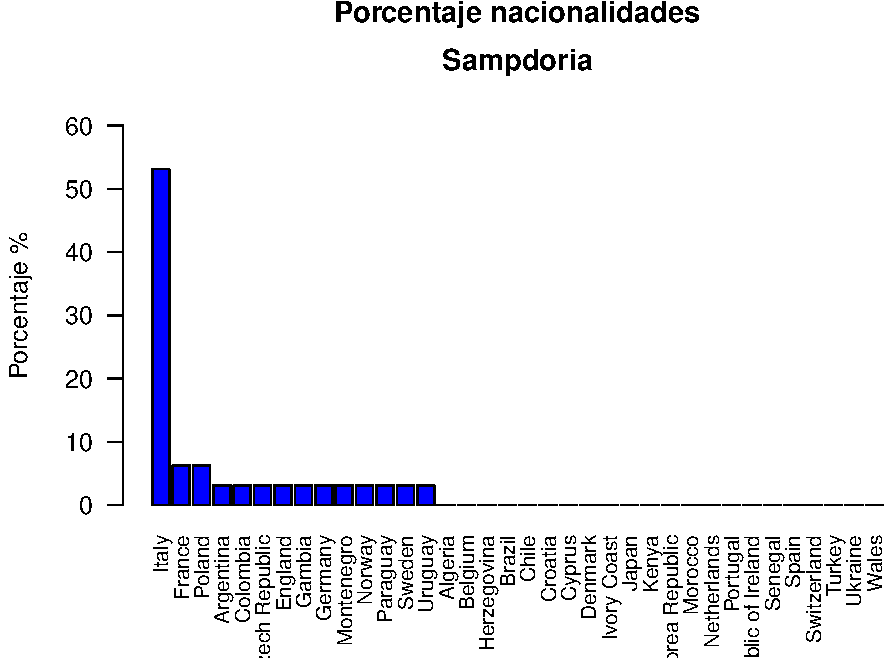
\includegraphics{taller_FIFA_SOLUCION_files/figure-latex/unnamed-chunk-9-5.pdf}
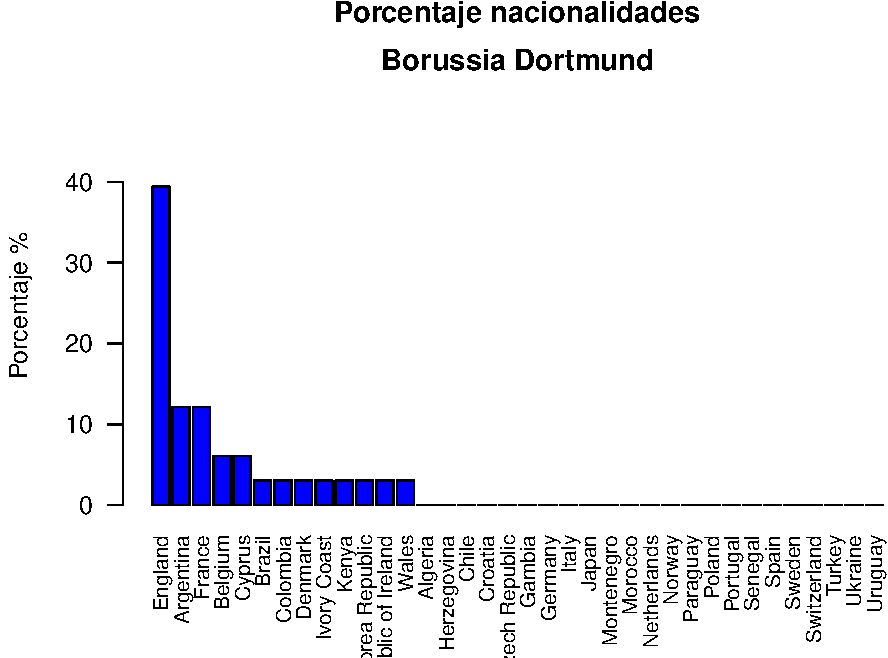
\includegraphics{taller_FIFA_SOLUCION_files/figure-latex/unnamed-chunk-9-6.pdf}

\begin{Shaded}
\begin{Highlighting}[]
\CommentTok{# paste0  concatena  caracteres sin espacio, paste es la función general}
\end{Highlighting}
\end{Shaded}

\hypertarget{pregunta-8}{%
\subsection{Pregunta 8}\label{pregunta-8}}

Encuentra la función (lineal, exponencial o potencial) que mejor
describe la dependencia funcional del sueldo de los jugadores en función
de la variable \texttt{shooting} en el data frame
\texttt{fifa20\_best\_shooting}. Representa dicha función junto con los
puntos (shooting, sueldo) en escala lineal.

\hypertarget{soluciuxf3n-7}{%
\subsubsection{Solución}\label{soluciuxf3n-7}}

Hay que seguir los pasos de la lección
\href{https://aprender-uib.github.io/AprendeR1/chap-lm.html}{Un
aperitivo: Introducción a la regresión linea: AprendeR1}

\begin{Shaded}
\begin{Highlighting}[]
\KeywordTok{summary}\NormalTok{(}\KeywordTok{lm}\NormalTok{(wage_eur}\OperatorTok{~}\NormalTok{shooting,}\DataTypeTok{data=}\NormalTok{fifa20_best_shooting))}\OperatorTok{$}\NormalTok{r.squared }\CommentTok{# lineal}
\end{Highlighting}
\end{Shaded}

\begin{verbatim}
## [1] 0.3650403
\end{verbatim}

\begin{Shaded}
\begin{Highlighting}[]
\KeywordTok{summary}\NormalTok{(}\KeywordTok{lm}\NormalTok{(}\KeywordTok{log10}\NormalTok{(wage_eur)}\OperatorTok{~}\KeywordTok{log10}\NormalTok{(shooting),}\DataTypeTok{data=}\NormalTok{fifa20_best_shooting))}\OperatorTok{$}\NormalTok{r.squared }\CommentTok{# potencial}
\end{Highlighting}
\end{Shaded}

\begin{verbatim}
## [1] 0.3334074
\end{verbatim}

\begin{Shaded}
\begin{Highlighting}[]
\KeywordTok{summary}\NormalTok{(}\KeywordTok{lm}\NormalTok{(}\KeywordTok{log10}\NormalTok{(wage_eur)}\OperatorTok{~}\NormalTok{shooting,}\DataTypeTok{data=}\NormalTok{fifa20_best_shooting))}\OperatorTok{$}\NormalTok{r.squared }\CommentTok{# exponencial}
\end{Highlighting}
\end{Shaded}

\begin{verbatim}
## [1] 0.3668289
\end{verbatim}

El mejor modelo es el que tenga mejor \(r.squared\) que es (por muy muy
poco ) el exponencial

\begin{Shaded}
\begin{Highlighting}[]
\KeywordTok{lm}\NormalTok{(}\KeywordTok{log10}\NormalTok{(wage_eur)}\OperatorTok{~}\NormalTok{shooting,}\DataTypeTok{data=}\NormalTok{fifa20_best_shooting)}
\end{Highlighting}
\end{Shaded}

\begin{verbatim}
## 
## Call:
## lm(formula = log10(wage_eur) ~ shooting, data = fifa20_best_shooting)
## 
## Coefficients:
## (Intercept)     shooting  
##     3.35568      0.02199
\end{verbatim}

luego

\[\log_{10}(wage\_eur)=  0.02418 \cdot shooting + 3.15960.\]
\[wage\_eur=  10^{3.15960}\cdot  10^{0.02418\cdot shooting}  .\]

Simplificando \(10^{0.02418}\approx1.0573\) y
\(10^{0.02418}\approx1444.1091\). Luego el modelo exponencial es

\[wage\_eur=  1444.1091\cdot 1.0573^{shooting}.\]

Con estos datos podemos dibujar la gráfica con la curva y los datos

\begin{Shaded}
\begin{Highlighting}[]
\NormalTok{potencial=}\ControlFlowTok{function}\NormalTok{(x) \{}\FloatTok{1444.1091}\OperatorTok{*}\StringTok{ }\FloatTok{1.0573}\OperatorTok{^}\NormalTok{x\}}
\KeywordTok{plot}\NormalTok{(fifa20_best_shooting}\OperatorTok{$}\NormalTok{shooting,fifa20_best_shooting}\OperatorTok{$}\NormalTok{wage_eur,}
     \DataTypeTok{xlim=}\KeywordTok{c}\NormalTok{(}\DecValTok{0}\NormalTok{,}\DecValTok{100}\NormalTok{),}\DataTypeTok{ylab=}\StringTok{"wage_eur"}\NormalTok{,}\DataTypeTok{xlab=}\StringTok{"shooting"}\NormalTok{,}\DataTypeTok{main=}\StringTok{"Curva potencial entre wage_eur y shooting"}\NormalTok{)}
\KeywordTok{curve}\NormalTok{(}\KeywordTok{potencial}\NormalTok{(x),}\DataTypeTok{col=}\StringTok{"red"}\NormalTok{,}\DataTypeTok{add =} \OtherTok{TRUE}\NormalTok{,}\DataTypeTok{xlim=}\KeywordTok{c}\NormalTok{(}\DecValTok{0}\NormalTok{,}\DecValTok{100}\NormalTok{))}
\end{Highlighting}
\end{Shaded}

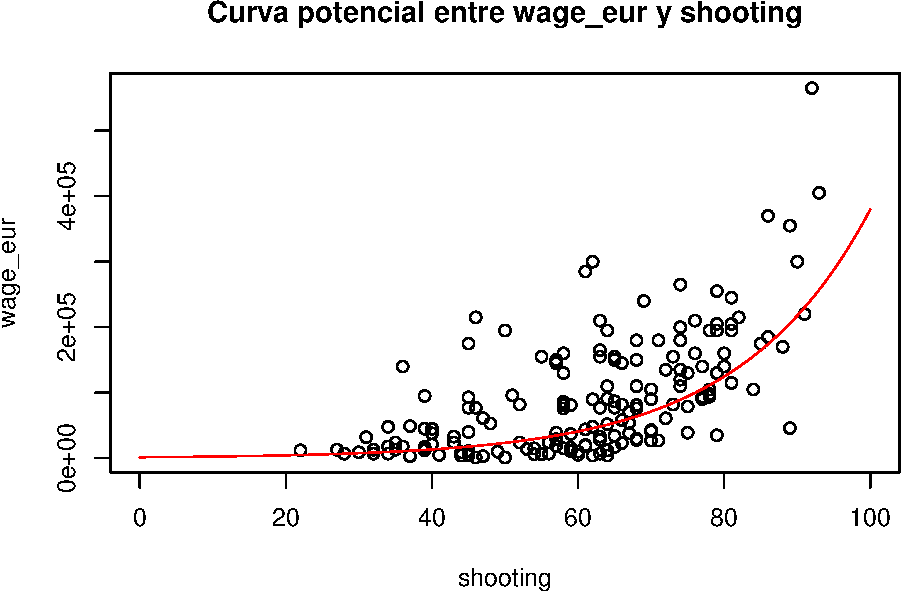
\includegraphics{taller_FIFA_SOLUCION_files/figure-latex/unnamed-chunk-12-1.pdf}

\end{document}
